\subsection{Articolo}
% link articolo:
% http://www.f1world.it/2016/06/f1-gp-europa-2016-qualifiche-emozioni-al-cardioplama-regalano-la-pole-a-nico-rosberg/
Verr\`a eseguita l'analisi di un articolo presente nel sito.

\begin{figure}[h] % 'h' not 'H'
  \centering
  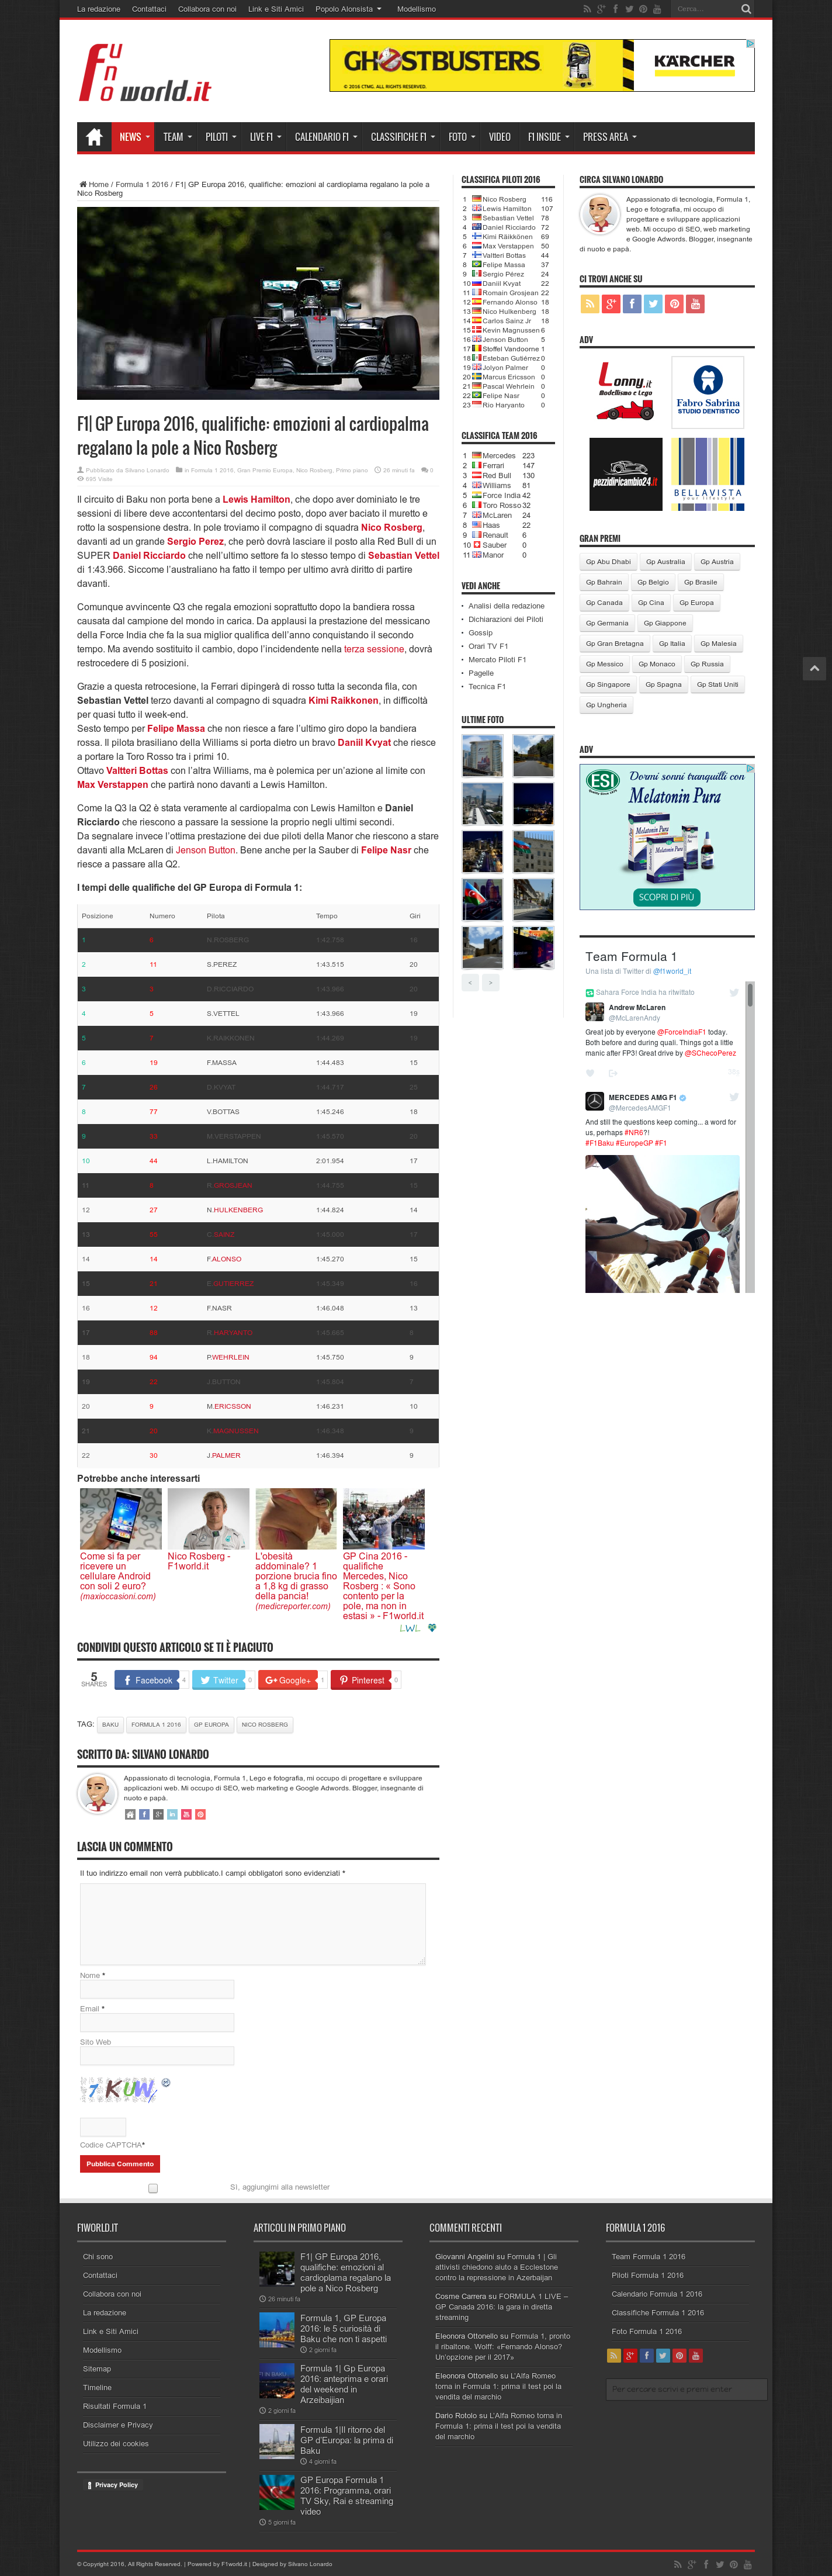
\includegraphics[height=18cm, width=10cm]{res/img/Article}
  \caption{\textit{Screenshot} di un articolo}
\end{figure}

Ancora una volta si fa notare come sia stata data importanza all'immagine che al
testo: è presente infatti subito dopo il menù un'immagine di apertura, che va
ad occupare la parte iniziale dell'articolo.
Di seguito si trova la descrizione testuale, che presenta una buona suddivisione
e distribuzione del contenuto, dove sono presenti link e parole chiave segnate
in grassetto.

In fondo all'articolo è presente una tabella, che non risulta essere molto
leggibile per via della scelta dei colori. Questa tabella inoltre risulta essere
spaziosa, aumentando il numero di scroll per scorrere la pagina.

Alla fine del contenuto è presente uno spazio riservato ad articoli relazionati.
È possibile notare come all'interno di questa sezione siano presenti inserzioni
pubblicitarie, che sono integrate in maniera omogenea per il tema, ma per i
contenuti non corrispondono agli argomenti del sito web.

È possibile condividere l'articolo nei social network più famosi, e prima della
sezione riservata ai commenti è presente una biografia dell'autore: questa
biografia è ripetuta anche nella parte iniziale della pagina, sulla destra.
Questa ripetizione secondo me è eccessiva e andrebbe eliminata.

La zona commenti consiste in un \textit{form} in cui è possibile commentare
senza essere registrati. I commenti poi verranno visualizzati dal più recente
al più vecchio.
